\apendice{Documentación técnica de programación}

\section{Introducción}

\section{Estructura de directorios}

Los directorios del proyecto son:

\dirtree{%
.1 /.
.2 doc.
.3 design.
.3 img.
.3 tex.
.2 research.
.3 data.
.3 model.
.3 src.
.4 Análisis de proyecciones.
.4 images.
.4 One-Class.
.3 tests.
.4 samples.
.5 input.
.5 output.
.2 smartbeds.
.3 api.
.3 bed.
.3 process.
.3 resources.
.4 assets.
.5 css.
.5 html.
.6 auth.
.6 components.
.5 img.
.5 js.
.3 routes.
.3 test.
}

En la carpeta \textit{\textbf{doc}} se encuentra toda la documentación de este proyecto. En \textit{\textbf{research}} están los ficheros de la investigación, dentro de esta están \textit{\textbf{data}}\footnote{Esta carpeta no se encuentra en el repositorio \textit{GitHub} porque contienen datos privados} que contiene los datos proporcionados para realizar el estudio, \textit{\textbf{model}} con los modelos binarios, \textit{\textbf{src}} con los ficheros fuentes y los \textit{Jupyter Notebooks} con la investigación y en \textit{\textbf{tests}} con los tests sobre algunas fuentes.

La carpeta \textbf{\textit{smartebs}} están las fuentes de la aplicación web siendo el modulo raíz. Dentro de esta están los módulo \textit{\textbf{api}} con la \texttt{API} web, \textit{\textbf{process}} con los algoritmos de procesamiento de los datos, \textit{\textbf{resources}} con la configuración y los \textit{assets} de la página web (plantillas, códigos \textit{JavaScript} etc), \textit{\textbf{routes}} que engloba las rutas \textit{URI} para dirigir las peticiones. Por último, está la carpeta \textit{\textbf{test}} con las pruebas unitarias.

De manera especial se encuentra la carpeta \textit{\textbf{bed}} dentro de \textbf{\textit{smartbeds}} que contiene un \textit{script} para la simulación de camas.
\section{Manual del programador}

\subsection{API}
Para proveer los servicios de esta aplicación a nuevos entornos se incorpora una API para utilizar los diferentes servicios del sistema especificados en los Casos de Uso, sección~\ref{casos-uso}.

El funcionamiento general de la API serán peticiones \texttt{POST} mediante \texttt{application/x-www-form-urlencoded} ante rutas específicas con los datos requeridos para cada petición. Y según sea el caso el servidor contestará con un fichero \texttt{JSON} con la respuesta adecuada. De manera particular está el sistema en tiempo real que funciona mediante mensajes de \textit{WebSockets}~\cite{wiki:websocket} usando la librería \textit{SocketIO}~\cite{tool:socketio} mediante la serie de eventos de la Figura~\ref{fig:ws-secuence}

\begin{figure}
	\centering
	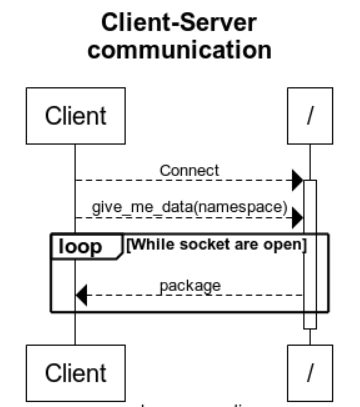
\includegraphics[width=0.7\textwidth]{img/ws-secuence.png}
	\caption{Comunicación cliente servidor \textit{websocket}}
	\label{fig:ws-secuence}
\end{figure}

Todas las respuestas del servidor contendrán los siguientes campos
\begin{lstlisting}[language=JSON]
{
  "status": 200|400|401|403|404|418|500,
  "message": "OK"|"Error description"
}
\end{lstlisting}

El valor de \texttt{status} tendrá un valor según los códigos HTTP definidos en el RFC 7231~\cite{RFC7231} y el mensaje será una explicación detallada del error producido.

Las distintas peticiones se especifican en la tabla \ref{tabla:api-specs2}

\begin{center}\small
	\tablefirsthead{
		\toprule
		\textbf{CU}	&	\textbf{URI}	&	\textbf{Petición}	&	\textbf{Respuesta} \\
		\otoprule
	}
	\tablehead{
		\multicolumn{4}{l}{\small\sl continúa desde la página anterior}\\
		\toprule
		\textbf{CU}	&	\textbf{URI}	&	\textbf{Petición}	&	\textbf{Respuesta} \\
		\otoprule
	}
	\tabletail{
		\hline
		\multicolumn{4}{r}{\small\sl continúa en la página siguiente}\\
	}
	\tablelasttail{
		\hline
	}
	\bottomcaption{Especificaciones del API}
	\begin{xtabular}{p{0.095\textwidth} p{0.2\textwidth} p{0.37\textwidth} p{0.33\textwidth}}
		CU-1		&	\texttt{/api/auth}	& \begin{lstlisting}[language=JSONT]
"user": text,
"pass": text
\end{lstlisting}&\begin{lstlisting}[language=JSONT]
{
  ...,
  "token": text,
  "role": text,
  "username": text
}\end{lstlisting}
\\
CU-2.1  CU-4		&	\texttt{/api/beds}	& 
\begin{lstlisting}[language=JSONT]
"token": text
\end{lstlisting}
&
\begin{lstlisting}[language=JSONT]
...,
"beds": [{
  	"bed_name": text,
	"ip_group": text,
	"port": text,
	"MAC": text,
	"UUID": text
    }
    ...]
\end{lstlisting}
\\\hubu
CU-2.2		&	\texttt{/api/bed}	& 
\begin{lstlisting}[language=JSONT]
token=text&
bedname=text
\end{lstlisting}
&
\begin{lstlisting}[language=JSONT]
{
  ...,
  "namespace": text
}\end{lstlisting}
\\\hubu
CU-2.2		&	\texttt{/} \textit{(WebSocket)}	& 
\begin{lstlisting}[language=JSONT]
{
   "namespace": namespace
}
\end{lstlisting}
&
\begin{lstlisting}[language=JSONT]
{
  "results": [result, prob, press_state, hr_state],
  "instance": datetime
  "vital": [HR,RR,SV,HRV,B2B],
  "pressure": [P1,P2,..,P6] 
}\end{lstlisting}
\\
CU-3		&	\texttt{/api/users}	& 
\begin{lstlisting}[language=JSONT]
token=text
\end{lstlisting}
&
\begin{lstlisting}[language=JSONT]
{
  ...,
  "users":[text,...,text]
}\end{lstlisting}
\\\hubu
CU-3.1		&	\texttt{/api/user/add}	& 
\begin{lstlisting}[language=JSONT]
token=text&
username=text&
password=text&
password-re=text
\end{lstlisting}
&
\begin{lstlisting}[language=JSONT]
{
  ...
}\end{lstlisting}
\\\hubu
CU-3.2		&	\texttt{/api/user/mod}	& 
\begin{lstlisting}[language=JSONT]
token=text&
username=text&
password=text&
password-re=text
[&pasword-old=text]
\end{lstlisting}
&
\begin{lstlisting}[language=JSONT]
{
  ...
}\end{lstlisting}
\\\hubu
CU-3.3		&	\texttt{/api/user/del}	& 
\begin{lstlisting}[language=JSONT]
token=text&
username=text
\end{lstlisting}
&
\begin{lstlisting}[language=JSONT]
{
    ...
}\end{lstlisting}
\\\hubu
CU-4.1		&	\texttt{/api/bed/add}	& 
\begin{lstlisting}[language=JSONT]
token=text&
bed_name=text&
ip_group=text&
port=text&
MAC=text&
UUID=text
\end{lstlisting}
&
\begin{lstlisting}[language=JSONT]
{
  ...
}\end{lstlisting}
\\\hubu
CU-4.2		&	\texttt{/api/bed/mod}	& 
\begin{lstlisting}[language=JSONT]
token=text&
bed_name=text&
ip_group=text&
port=text&
MAC=text&
UUID=text
\end{lstlisting}
&
\begin{lstlisting}[language=JSONT]
{
  ...
}\end{lstlisting}
\\\hubu
CU-4.3		&	\texttt{/api/bed/del}	& 
\begin{lstlisting}[language=JSONT]
token=text&
bed_name=text
\end{lstlisting}
&
\begin{lstlisting}[language=JSONT]
{
  ...
}\end{lstlisting}
\\\hubu
CU-4.4		&	\texttt{/api/bed/perm}	& 
\begin{lstlisting}[language=JSONT]
token=text&
mode=[info|change]
[&bed_name=text&
username=text]
\end{lstlisting}
&
\begin{lstlisting}[language=JSONT]
{
  ...,
  "permission":[
   {
    "username":text,
    "bed_name":text
   },
   ...
  ]
}\end{lstlisting}
\\\bottomrule
	\end{xtabular}
	\label{tabla:api-specs2}
\end{center}

\section{Compilación, instalación y ejecución del proyecto}

Este proyecto contiene un servidor web, sobre el cual se explicará su proceso de despliegue en este apartado. Sin embargo, no disponemos de camas reales que puedan aportar datos en tiempo real como hemos visto en la figura~\ref{fig:componentes} debido a que este \textit{hardware} es privado.

En su lugar se ha creado un \textit{script} de \textit{Python} que emite cada 0,4 segundos de manera indefinida datos que se han obtenido previamente. Este \textit{script} se encuentra en la carpeta \texttt{smartbeds/bed}.


\subsection{Requisitos del sistema}

Para el funcionamiento correcto de la aplicación se requiere de \textit{hardware} los siguientes mínimos:

\begin{itemize}
	\item \textbf{Procesador}: arquitectura de 64 bits con soporte multihilo. Se recomienda un mínimo de 1,5 GHz, 16MiB de memoria caché y dos núcleos.
	\item \textbf{Memoria}: 768MiB, incorporando 256MiB aprox. por cada nueva cama incorporada. 
	\item \textbf{Almacenamiento}: 16MiB aprox.
\end{itemize}

\subsection{Requisitos software}

Para poder ejecutar la aplicación se necesitan los siguientes apartados de software.

Entorno \textit{Python}, versión 3.7 con las librerías de \textit{requeriments.txt} instaladas (\texttt{pip install -r requeriments.txt}).
Base de datos \textit{MySQL} o con API compatible como \textit{MariaDB}. Servidor web con soporte de \textit{proxy} reverso y \textit{websokets} como \textit{Nginx} versión 1.16.

\subsection{Instalación en entorno GNU/Linux}

El primer paso necesario es la configuración de la base de datos en la cual se van a almacenar los datos del sistema. La estructura de esta base de datos se encuentra en el fichero \texttt{/smartbeds/resources/database.sql}. Tras esto es necesario crear el fichero \texttt{/smartbeds/resources/project.json} que tendrá la configuración de la aplicación siguiendo este formato:

\begin{lstlisting}[language=JSON]
{
	"secret-key": "clave secreta",
	"url":  "http://127.0.0.1",
	"port": 3031,
	"mode": "ssl"
	"database": {
		"host": "database-host",
		"database": "database-name",
		"user": "database-user",
		"password": "database-password"
	}
}
\end{lstlisting}

En cada campo habría que incorporar los cambios oportunos y se recomienda no modificar el campo \texttt{url}. De manera especial el campo mode puede ser \texttt{ssl} o \texttt{no-ssl} si los \textit{websockets} se ejecutan sobre \textit{SSL} o no. Tras esto ya el programa es ejecutable y puede funcionar al ejecutar el fichero \texttt{/index.py}.

El siguiente paso es crear la configuración del servidor \textit{HTTP} para redirigir las peticiones externas a la aplicación local. Como ejemplo, para un servidor \textit{Nginx} la configuración sería la siguiente:

\begin{lstlisting}[language=JSON]
server {
	listen 443 ssl http2;
	server_name $server_name$;
	root $route$;
	
	location / {
		include proxy_params;
		proxy_pass http://127.0.0.1:3031;
	}
	
	location /socket.io {
		include proxy_params;
		proxy_http_version 1.1;
		proxy_buffering off;
		proxy_set_header Upgrade $http_upgrade;
		proxy_set_header Connection "Upgrade";
		proxy_pass http://127.0.0.1:3031/socket.io;
	}
}
\end{lstlisting}

Siendo necesario modificar el nombre del servidor por el dominio o ip de acceso y la raíz como la ruta donde se encuentra el fichero \texttt{index.py}, aunque esto último no es necesario para el funcionamiento, solo como referencia interna.

Por último es necesario crear un demonio de \texttt{systemd} que ejecute la aplicación en segundo plano. El fichero de configuración de este demonio se alojaría en \texttt{/usr/lib/systemd/system/smartbeds.service}. Siendo el fichero en cuestión semejante a:
\begin{lstlisting}[language={Ini}]
[Unit]
Description=Smartbed Service
After=network.target
StartLimitIntervalSec=0

[Service]
Type=simple
Restart=always
RestartSec=1
User=http
WorkingDirectory=/ruta/a/la/carpeta
ExecStart=python index.py

[Install]
WantedBy=multi-user.target
\end{lstlisting}

El campo \texttt{ExecStart} podría cambiar en el caso de utilizar algún entornos \textit{Python} como son los que provee conda. En el caso de ser así se recomienda cambiar el campo por \texttt{bash index.sh} siendo el fichero semejante a:

\begin{lstlisting}[language=bashb]
#!/bin/bash
/opt/miniconda3/envs/entorno/bin/python index.py
\end{lstlisting}

Finalmente solo hace falta lanzar el demonio con el comando \texttt{systemctl start smartbeds}.

\section{Pruebas del sistema}
